Dans cette phase nous allons présenter le diagramme de cas d’utilisation de ce sprint. Ensuite, nous mettons en disposition les descriptions textuelles de certains cas d’utilisation.
\subsubsection{ Diagramme de cas d’utilisation du sprint 2.1}
    La figure \ref{fig:caseS21} illustre le diagramme de cas d’utilisation pour le sprint 2.1.
        \begin{figure}[H]
            \centering
            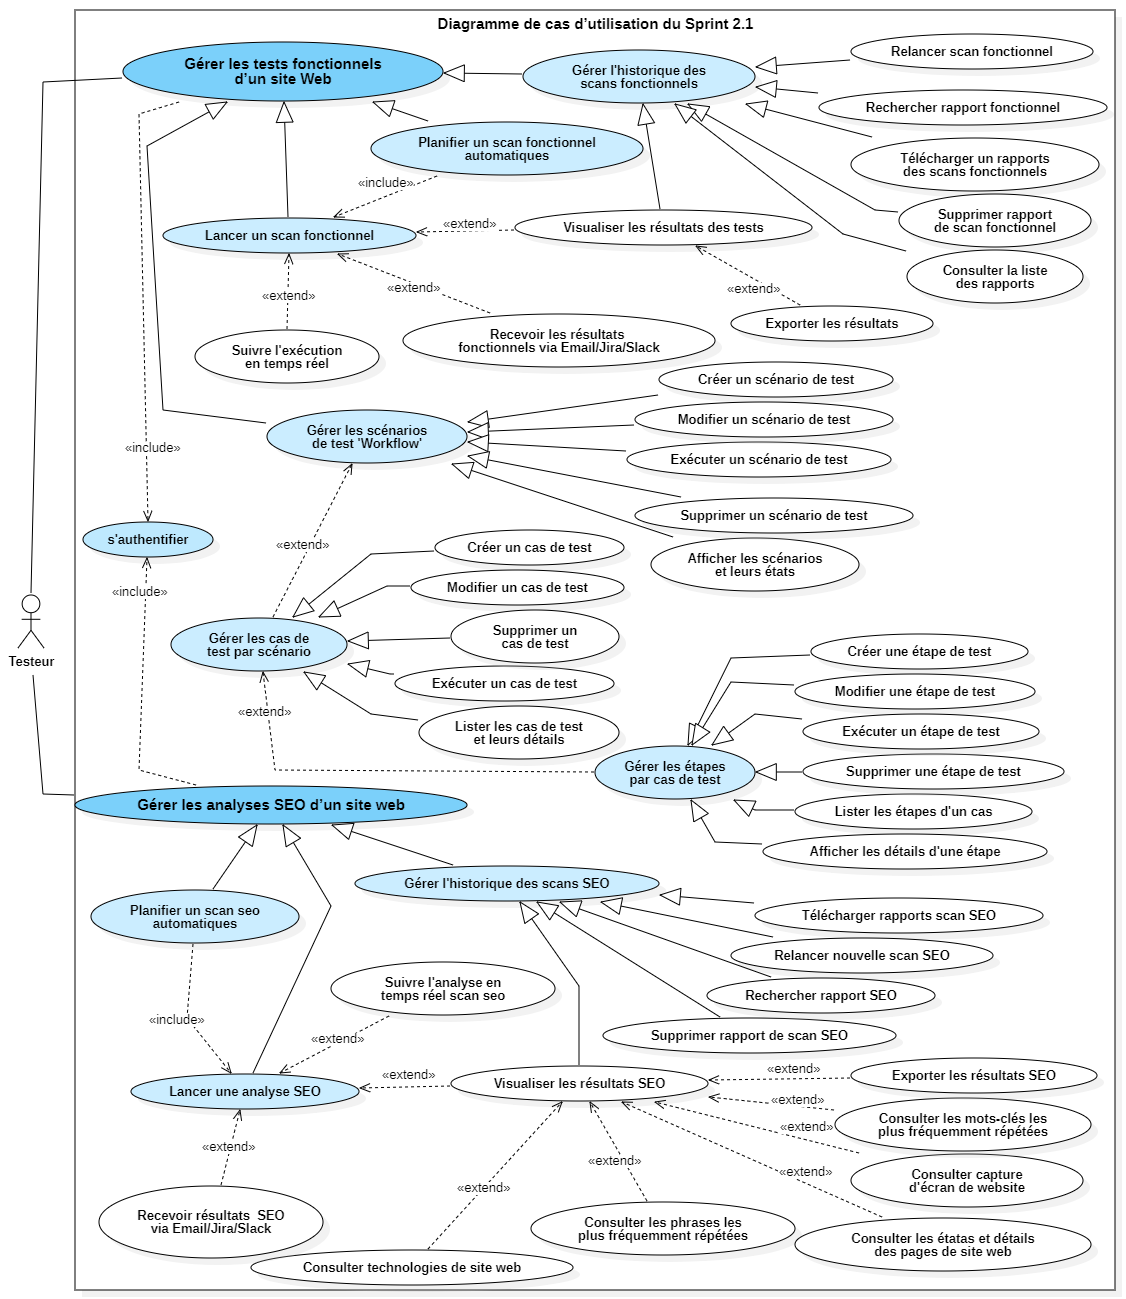
\includegraphics[width=\linewidth]{chapitres/ch4Sp2/section/sprint2.1/img/LastUseCaseSprint2.1.png}
            \caption{Diagramme de cas d'utilisations du sprint 2.1}
            \label{fig:caseS21}
        \end{figure}
\subsection{Raffinement des cas d'utilisation}
    \subsubsection{Description textuelle du cas d'utilisation « Lancer un scan fonctionnel »}
        Le tableau ~\ref{tab:descScanFonctionnel} présente la description textuelle du cas d'utilisation "Lancer un scan fonctionnel".
                \begin{spacing}{1}
                    \begin{longtable}{|p{0.12\linewidth}|p{0.85\linewidth}|}
                        \caption{Description textuelle du cas d'utilisation : Lancer un scan fonctionnel}
                        \label{tab:descScanFonctionnel}\\
                        \hline
                        \textbf{Titre} & Lancer un scan fonctionnel \\
                        \hline
                        \textbf{Acteur} & Testeur \\
                        \hline
                        \textbf{Résumé} & Ce cas d'utilisation permet au testeur de déclencher l'exécution automatisée d'un ensemble de scénarios de test fonctionnels sur une application web afin de valider le comportement de l'application avec un suivi en temps réel. \\
                        \hline
                        \textbf{Pré-conditions} & 
                        \begin{minipage}{0.83\textwidth}
                             \vspace{0.05cm}
                            \begin{itemize}[left=0cm]
                                \item[\textbullet] L'utilisateur est authentifié en tant que Testeur
                                \item[\textbullet] Au moins un scénario de test existe dans le système
                            \end{itemize}
                        \end{minipage} \\
                        \hline
                        \textbf{Post-conditions} & 
                        \begin{minipage}{0.83\textwidth}
                            \vspace{0.1cm}
                            \textbf{En cas de succès :}
                            \begin{itemize}[left=0cm]
                                \item[\textbullet] Le scan fonctionnel est lancé avec succès avec un identifiant unique de scan est généré
                                \item[\textbullet] Les notifications sont envoyées selon la configuration
                                \item[\textbullet] L'historique est mis à jour
                            \end{itemize}
                            \textbf{En cas d'échec :}
                            \begin{itemize}[left=0cm]
                                \item[\textbullet] Le scan n'est pas lancé et un message d'erreur explicite est affiché
                                \item[\textbullet] Aucune notification n'est envoyée
                            \end{itemize}
                            \vspace{0.1cm}
                        \end{minipage} \\
                        \hline
                        \textbf{Scénario nominal} & 
                        \begin{minipage}{0.83\textwidth}
                            \vspace{0.1cm}
                            \begin{enumerate}[label=\arabic*.]
                                \item Le testeur accède à l'interface de lancement de scan
                                \item Le système affiche les scénarios disponibles
                                \item Le testeur sélectionne les scénarios à exécuter.
                                \item Le testeur confirme le lancement
                                \item Le système génère un ID unique, crée une session d'exécution et met à jour le statut à "En cours"
                                \item Le système envoie les notifications de début
                                \item Le système lance l'exécution des tests en arrière-plan
                                \item Le système active le suivi en temps réel
                                \item Si l'envoi des rapports est configuré, le système crée automatiquement des tickets Jira ou envoie un message via Slack ou par email, selon le type de configuration.
                            \end{enumerate}
                            \vspace{0.1cm}
                        \end{minipage}\\
                        \hline
                        \textbf{Scénario d'erreur} &
                        \begin{minipage}{0.83\textwidth}
                            \vspace{0.1cm}
                            \begin{itemize}[left=0cm]
                                \item[\textbullet] \textbf{Étape 3 (Aucun scénario sélectionné):}
                                \begin{itemize}[label=\ding{56}]
                                    \item Le système affiche un message d'erreur
                                    \item Le système invite le testeur à sélectionner au moins un scénario
                                    \item Retour à l'étape 3
                                \end{itemize}
                            \end{itemize}
                            \vspace{0.1cm}
                        \end{minipage}\\
                        \hline
                    \end{longtable}
                \end{spacing}   
    \vspace{-0.2cm}
    \subsubsection{Description textuelle du cas d’utilisation «Lancer une analyse SEO»}    
            Le tableau ~\ref{tab:descAnalyseSEO} présente la description textuelle du cas d’utilisation "Lancer une analyse SEO".
            \begin{spacing}{1.2}
                \begin{longtable}{|p{0.12\linewidth}|p{0.85\linewidth}|}
                \caption{Description textuelle du cas d’utilisation : Lancer une analyse SEO}
                \label{tab:descAnalyseSEO}\\
                \hline
                \textbf{Titre} & Lancer une analyse SEO\\ 
                \hline
                \textbf{Acteur} & Testeur \\
                \hline
                \textbf{Résumé} & Ce cas d'utilisation permet au testeur de lancer une analyse d'un site web afin d'évaluer sa qualité SEO à travers différents indicateurs techniques et de contenu. \\
                \hline
                \textbf{Pré-conditions} &
                Le testeur doit avoir accès à l’interface de scan, et l’URL du site cible doit être valide et accessible publiquement. \\
                \hline
                \textbf{Post-conditions} &
                Un rapport SEO est généré, incluant les résultats de l’analyse (balises, mots clés, performances…) et un score global est calculé. \\
                \hline
                \textbf{Scénario nominal} &
                \begin{minipage}{0.83\textwidth}
                \vspace{0.1cm}
                \begin{enumerate}[label=\arabic*.]
                \item Le testeur accède à l’interface d’analyse SEO.
                \item Il saisit ou colle l’URL du site à analyser.
                \item Il lance l’analyse en cliquant sur le bouton dédié.
                \item Le système récupère les données du site (HTML, métadonnées, performances…).
                \item Le système effectue les vérifications SEO : balises manquantes, densité des mots clés, temps de chargement, structure, etc.
                \item Le système calcule un score global basé sur les critères définis.
                \item Un rapport d’analyse détaillé est généré et affiché à l’écran.
                \end{enumerate}
                \vspace{0.1cm}
                \end{minipage}\\
                \hline
                \textbf{Scénario d’erreur} &
                \begin{minipage}{0.83\textwidth}
                \vspace{0.1cm}
                \begin{itemize}[left=0cm]
                \item[\textbullet] \textbf{Étape 2 (URL invalide):}
                \begin{itemize}[label=\ding{56}]
                \item Le système affiche un message d’erreur indiquant que l’URL saisie est invalide.
                \end{itemize}
                    \item[\textbullet] \textbf{Étape 4 (Échec de récupération de données):}
                    \begin{itemize}[label=\ding{56}]
                        \item Le système affiche une alerte mentionnant l’échec de connexion au site ou un temps d’attente dépassé.
                    \end{itemize}
                
                    \item[\textbullet] \textbf{Étape 5 (Erreur d’analyse):}
                    \begin{itemize}[label=\ding{56}]
                        \item Si une erreur technique survient lors du parsing SEO, une notification avec détail de l’erreur est proposée au testeur.
                    \end{itemize}                  
                \end{itemize}
                \vspace{0.1cm}
                \end{minipage}\\
                \hline
                \end{longtable}
            \end{spacing}            
        \vspace{-0.3cm}